\mysection{Fonction toupper()}
\myindex{\CStandardLibrary!toupper()}

Une autre fonction courante transforme un symbole de minuscule en majuscule, si besoin:

\lstinputlisting[style=customc]{\CURPATH/toupper.c}

L'expression \TT{'a'+'A'} est laissée dans le code source pour améliorer la lisibilité,
elle sera optimisée par le compilateur, bien sûr.
\footnote{Toutefois, pour être méticuleux, il y a toujours des compilateurs qui ne
peuvent pas optimiser de telles expressions et les laissent telles quelles dans le
code.}.

Le code \ac{ASCII} de \q{a} est 97 (ou 0x61), et celui de \q{A}, 65 (ou 0x41).

La différence (ou distance) entre les deux dans la table \ac{ASCII} est 32 (ou 0x20).

Pour une meilleure compréhension, le lecteur peut regarder la table \ac{ASCII} 7-bit
standard:

\begin{figure}[H]
\centering
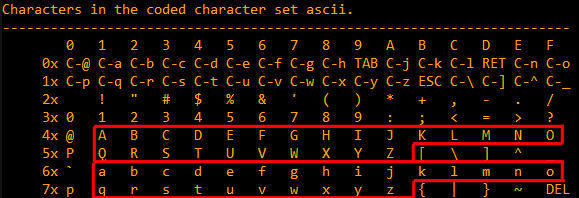
\includegraphics[width=0.8\textwidth]{ascii.png}
\caption{table \ac{ASCII} 7-bit dans Emacs}
\end{figure}

\subsection{x64}

\subsubsection{Deux opérations de comparaison}

MSVC \NonOptimizing est direct: le code vérifie si le symbole en entrée est dans
l'intervalle [97..122] (ou dans l'intervalle [`a'..`z']) et soustrait 32 si c'est
le cas.

Il y a quelques artefacts du compilateur:

\lstinputlisting[caption=MSVC 2013 (x64) \NonOptimizing,numbers=left,style=customasmx86]{\CURPATH/MSVC_2013_x64_FR.asm}

Il est important de remarquer que l'octet en entrée est chargé dans un slot 64-bit
de la pile locale à la ligne 3.

Tous les bits restants ([8..e3]) ne sont pas touchés, i.e., contiennent du bruit indéterminé
(vous le verrez dans le débogueur).

% TODO add debugger example
Toutes les instructions opèrent seulement au niveau de l'octet, donc c'est bon.

La dernière instruction \TT{MOVZX} à la ligne 15 prend un octet de la pile locale
et l'étend avec des zéro à un type de donnée \Tint 32-bit.

GCC \NonOptimizing fait essentiellement la même chose:

\lstinputlisting[caption=GCC 4.9 (x64) \NonOptimizing,style=customasmx86]{\CURPATH/GCC_49_x64_O0.s}

\subsubsection{Une opération de comparaison}
\label{toupper_one_comparison}

MSVC \Optimizing fait un meilleur travail, il ne génère qu'une seule opération de
comparaison:

\lstinputlisting[caption=MSVC 2013 (x64) \Optimizing,style=customasmx86]{\CURPATH/MSVC_2013_Ox_x64.asm}

Il a déjà été expliqué comment remplacer les deux opérations de comparaison par une
seule: \myref{one_comparison_instead_of_two}.

Nous allons maintenant récrire ceci en \CCpp:

\begin{lstlisting}[style=customc]
int tmp=c-97;

if (tmp>25)
        return c;
else
        return c-32;
\end{lstlisting}

La variable \emph{tmp} doit être signée.

Cela fait deux opérations de soustraction en cas de transformation plus une comparaison.

Par contraste, l'algorithme original utilise deux opérations de comparaison plus
une soustraction.

GCC \Optimizing est encore meilleur, il supprime le saut (ce qui est bien: \myref{branch_predictors})
en utilisant l'instruction CMOVcc:

\lstinputlisting[caption=GCC 4.9 (x64) \Optimizing,numbers=left,style=customasmx86,label=toupper_GCC_O3]{\CURPATH/GCC_49_x64_O3.s}

À la ligne 3 le code prépare la valeur soustraite en avance, comme si la conversion
avait toujours lieu.

À la ligne 5 la valeur soustraite dans EAX est remplacée par la valeur en entrée
non modifiée si la conversion n'est pas nécessaire.
Et ensuite cette valeur (bien sûr incorrecte) est abandonnée.

La soustraction en avance est le prix que le compilateur paye pour l'absence de saut
conditionnel.

\subsection{ARM}

Keil \Optimizing pour le mode ARM génère aussi une seule comparaison:

\lstinputlisting[caption=\OptimizingKeilVI (\ARMMode),style=customasmARM]{\CURPATH/Keil_ARM_O3.s}

\myindex{ARM!\Instructions!SUBcc}
\myindex{ARM!\Instructions!ANDcc}
Les instructions SUBLS et ANDLS ne sont exécutées que si la valeur dans \Reg{1} est
inférieure à 0x19 (ou égale).

Keil \Optimizing pour le mode Thumb génère lui aussi une seule opération de comparaison:

\lstinputlisting[caption=\OptimizingKeilVI (\ThumbMode),style=customasmARM]{\CURPATH/Keil_thumb_O3.s}

\myindex{ARM!\Instructions!LSLS}
\myindex{ARM!\Instructions!LSLR}
Les deux dernières instructions LSLS et LSRS fonctionnent comme \TT{AND reg, 0xFF}:
elles sont équivalentes à l'expression \CCpp $(i<<24)>>24$.

Il semble que Keil pour le mode Thumb déduit que ces deux instructions de 2-octets
sont plus courtes que le code qui charge la constante 0xFF dans un registre plus
une instruction AND.

\subsubsection{GCC pour ARM64}

\lstinputlisting[caption=GCC 4.9 (ARM64) \NonOptimizing,style=customasmARM]{\CURPATH/GCC_49_ARM64_O0.s}

\lstinputlisting[caption=GCC 4.9 (ARM64) \Optimizing,style=customasmARM]{\CURPATH/GCC_49_ARM64_O3.s}

\subsection{Utilisation d'opérations sur les bits}
\label{toupper_bit}

Étant donné le fait que le bit d'indice 5 (en partant depuis 0) est toujours présent
après le test, soustraire revient juste à effacer ce seul bit, mais la même chose
peut être effectuée avec un AND.

Encore plus simple, en XOR-ant:

\lstinputlisting[style=customc]{\CURPATH/toupper2.c}

Le code est proche de ce GCC avec optimisation a produit pour l'exemple précédent
(\myref{toupper_GCC_O3}):

\lstinputlisting[caption=GCC 5.4 (x86) \Optimizing,style=customasmx86]{\CURPATH/toupper2_GCC540_x86_O3.s}

\dots mais \INS{XOR} est utilisé au lieu de  \INS{SUB}.

Changer le bit d'indice 5 est juste déplacer un \textit{curseur} dans la table \ac{ASCII}
en haut ou en bas de deux lignes.

Certains disent que les lettres minuscules/majuscules ont été placées de cette façon
dans la table \ac{ASCII} intentionnellement, car:

\begin{framed}
\begin{quotation}
Very old keyboards used to do Shift just by toggling the 32 or 16 bit, depending on the key; this is why the relationship between small and capital letters in ASCII is so regular, and the relationship between numbers and symbols, and some pairs of symbols, is sort of regular if you squint at it.
\end{quotation}
\end{framed}

( Eric S. Raymond, \url{http://www.catb.org/esr/faqs/things-every-hacker-once-knew/} )

Donc, nous pouvons écrire ce morceau de code, qui change juste la casse des lettres:

\lstinputlisting[style=customc]{\CURPATH/flip_FR.c}

\subsection{Summary}

Toutes ces optimisations de compilateurs sont aujourd'hui courantes et un rétro-ingénieur
pratiquant voit souvent ce genre de patterns de code.
